\documentclass{aastex}
\begin{document}

\section{CX fit model}
Let $\psi_i$ denote the projectile state $i$, and $\chi_{nlj}$ denote the
charge exchange capture orbital. The final state after the capture can be
expressed as a linear mixing of the product of the two functions:
\begin{equation}
  \Psi_k = \sum_{i,nlj}b^k_{i,nlj}|\psi_i\chi_{nlj};\gamma\pi J>
\end{equation}
where $\pi$ and $J$ are the parity and total angular momentum of the product
state, and $\gamma$ represents all other quantum numbers required to fully
describe the state. Therefore, final state index $k$ represent a collection of
quantum numbers $i$, $nlj$, $\gamma$, $\pi$, and $J$. $b_{i,nlj}$ are the
mixing coefficients, which can be 
determined solving the atomic structure problem of the recombined
ion. Ignoring the interference terms, the charge exchange cross section from
the projectile state $\psi_i$ to the recombined state $\Psi_k$ can be
approximated as:
\begin{equation}
  \sigma_k = \sum_{nlj}|b^k_{i,nlj}|^2a_{i,nlj,\gamma\pi J}\sigma_{\alpha,nlj}
\end{equation}
where $a_{i,nlj,\gamma\pi J}$ are the angular momentum decoupling factors, and
$\sigma_{\alpha,nlj}$ is the charge exchange cross section to a one electron
orbital $\chi_{nlj}$, which may depend on a subset of the quantum numbers
describing the product state. For typical EBIT measurements on highly charged
ions, the only important initial state is the ground state $\psi_0$. Due to
configuration interaction mixing, the capture to core excited final state $k$
may have non-vanishing cross sections. However, the free parameters in our
model are the one-electron capture cross sections from the ground state, the
coefficients $b^k_{0,nlj}$ and $a_{0,nlj,\gamma\pi J}$ can all be calculated
from atomic structure codes.

In the most simple model, $\sigma_{\alpha,nlj}$ only depends on the
non-relativistic quantum numbers of the one-electron orbital $nl$, such that:
\begin{equation}
  \sigma_{\alpha,nlj} = \frac{2j+1}{4l+2}\sigma_{nl}
\end{equation}
For complex ions, this represent a huge reduction of number of free parameters
required to describe the detailed final state resolved capture cross
sections. For low energy charge exchange collisions, it is well known that the
capture is dominated by a few $n$ values around its maximum $n_{max}$. One can
further simplify the parametrization as
\begin{equation}
  \sigma_{nl} = \sigma_t\beta_nf_l
\end{equation}
where $\sigma_t$ is the total capture cross section, $\beta_n$ and $f_l$ are
the $n$ and $l$ distribution, respectively, where we assume $f_l$ is the same
for the few neighboring $n$ values that dominate the charge exchange
process. The complete factorization of the $n$ and $l$ distributions further
reduces the number of free parameters in the model. This procedure of reducing
the parameter space is very important to obtaining a physically meaningful
solution from the measured cascade spectra.

It is possible that the $n$ and $l$ distribution functions 
may have some dependence on certain quantum numbers of the projectile or
product state, such as total spin and total angular momenta. Therefore our
spectral basis set is comprised of a set of lines, where the intensity of the
$m$-th line can be written as:
\begin{equation}
I_m = A_{m,k}\sigma_k = B^{\gamma\pi J}_{m,nl}\beta^{\alpha}_nf^{\alpha}_l
\end{equation}
The matrix $A$, and therefore $B$ can be obtained by the radiative cascade
calculation.

In practice, I found that for CX of H-like ion, a set of $\beta_n$ amd $f_l$
parameters are enough to adqequately fit the measured spectra. for He-like
ions, choosing $\alpha = S$ as the total spin of the product state is
appropriate. To fit the Ne-like Ni spectra, it is required to choose $\alpha$
to the the combination of $S$ and $J$.

\ref{fig:s+he.spec} shows the fitted spectra of S+He charge
exchange. \ref{fig:s+he.nldist} shows the reconstructed $n$ and $l$
distribution of H-like, singlet He-like, and triplet He-like ions.
\begin{figure}
  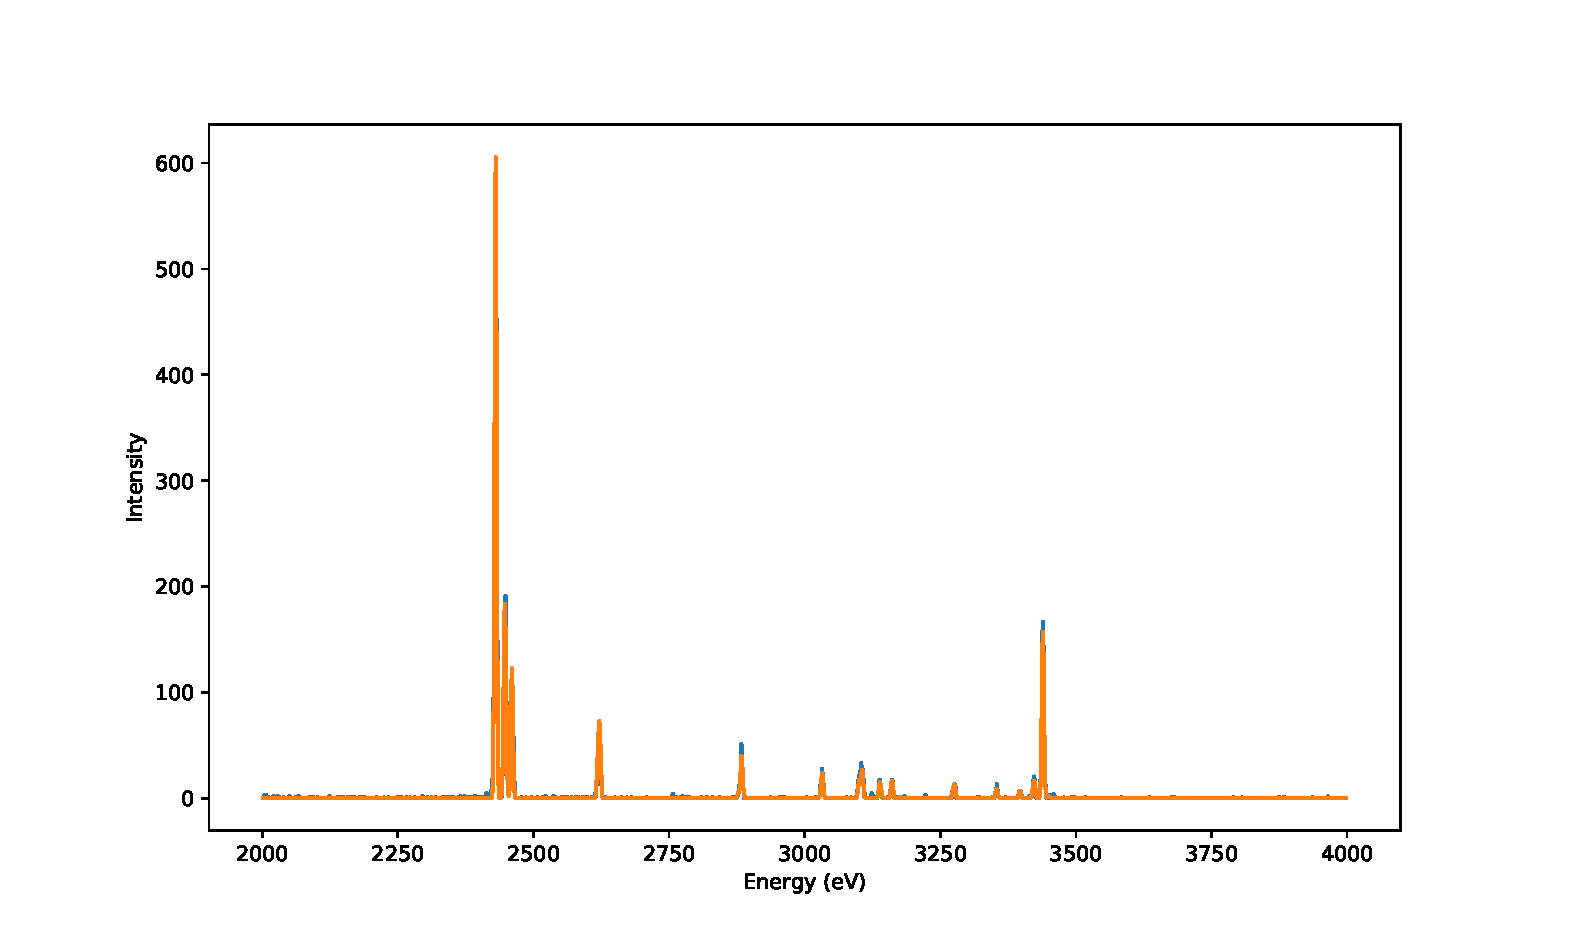
\includegraphics[width=5in]{spec_s_he.eps}
  \caption{\label{fig:s+he.spec}Model fit to the measured S+He charge exchange
    spectrum.}
\end{figure}

\begin{figure}
  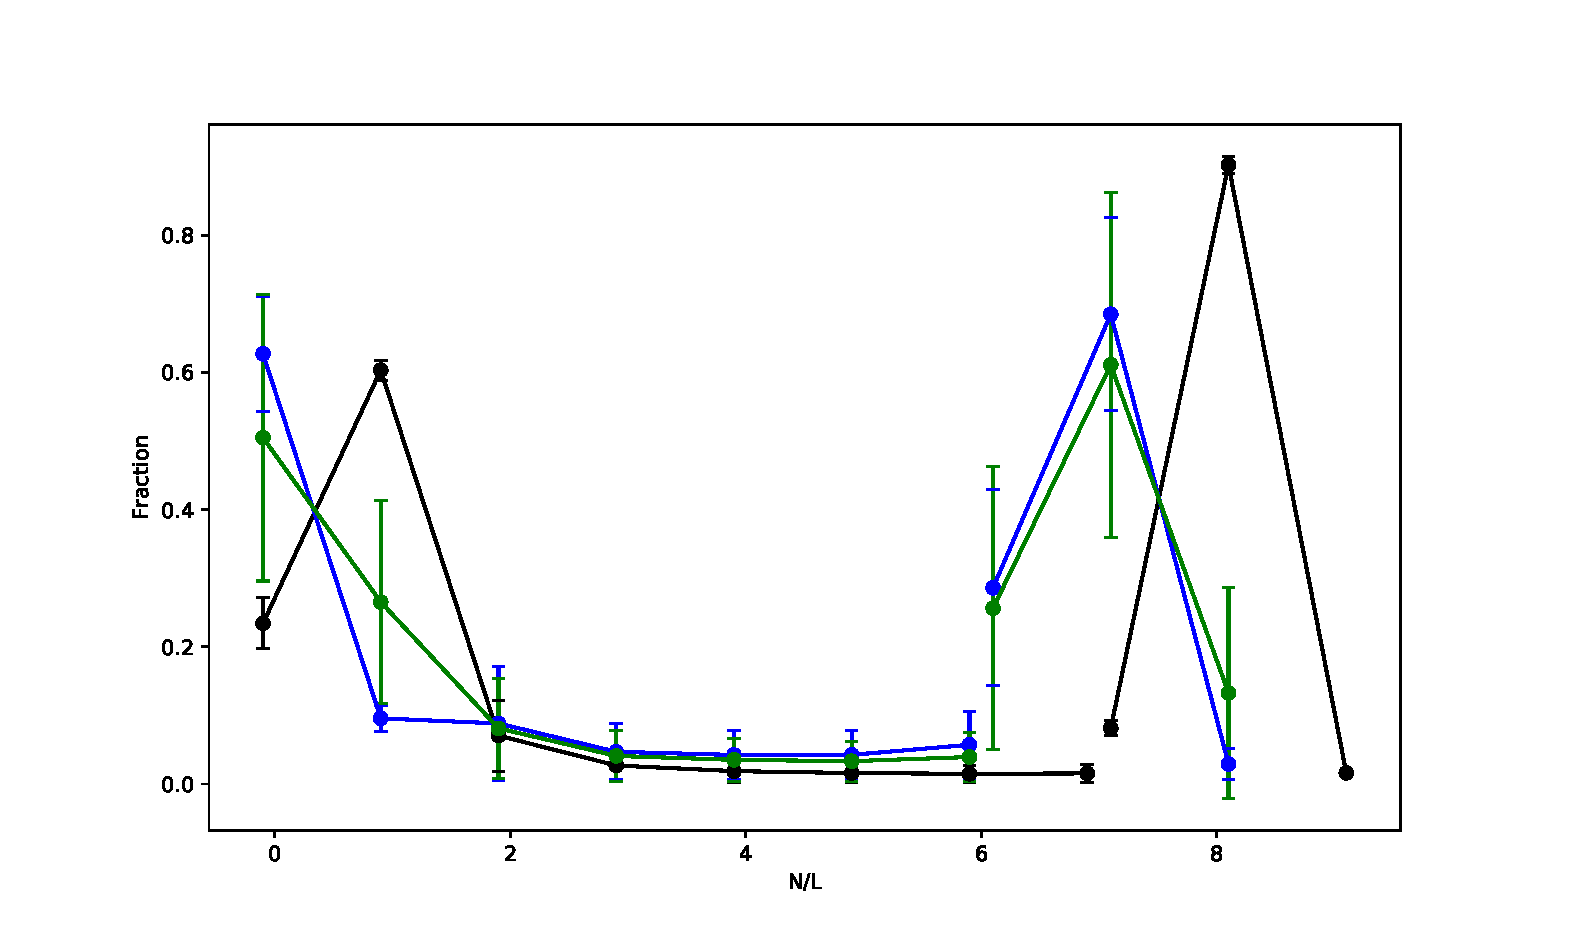
\includegraphics[width=5in]{nl_s_he.eps}
  \caption{\label{fig:s+he.nldist}Reconstructed $n$ and $l$ distributions of the
    H-like, singlet He-like and triplet He-like ions.}
\end{figure}

\ref{fig:ni+h2.spec} shows the fitted spectra of Ne-like Ni charge exchange
spectra. \ref{fig:ni+h2.zoom} shows the spectrum of weaker lines in more
detail. \ref{fig:ni+h2.nldist} shows the $n$ and $l$
distributions. \ref{fig:ni+h2.icx} shows the relative capture cross sections
to individual states with three core states of the F-like Ni. The core excited
state capture with a $2p_{1/2}$ hole is dominated by the $8p_{1/2}$ capture,
which interact with a $9p$ state in the ground core strongly. The core
excitation capture with a $2s$ hole is dominated by the $5d_{5/2}$ orbital,
which interact strongly with a $10p$ state with ground core.
\begin{figure}
  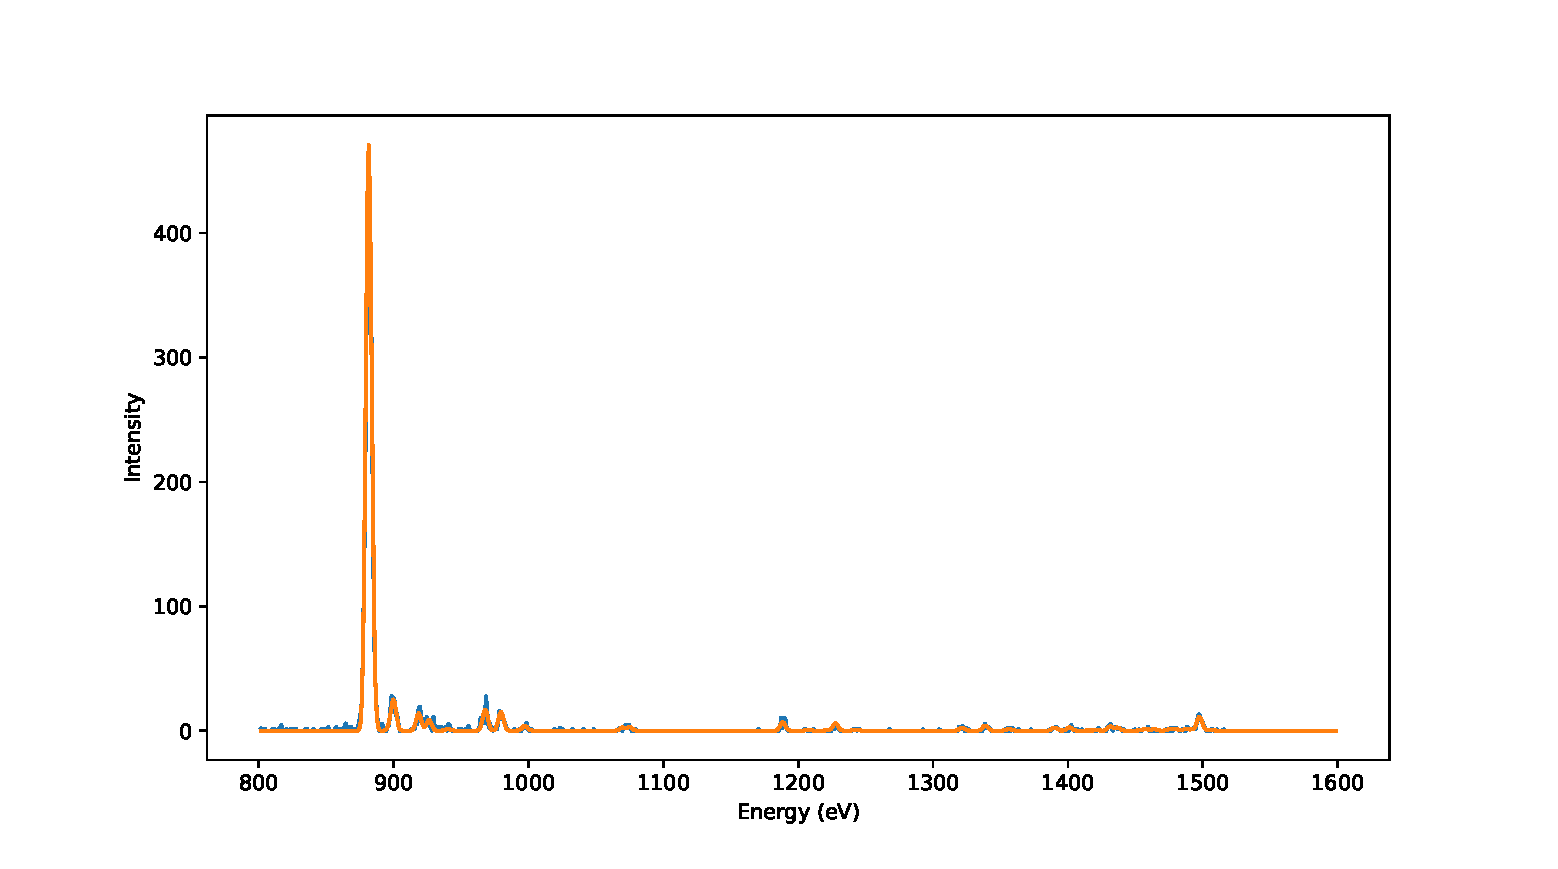
\includegraphics[width=5in]{spec_ni_h2.eps}
  \caption{\label{fig:ni+h2.spec}Model fit to the Ni+H2 charge exchange
    spectrum.}
\end{figure}
\begin{figure}
  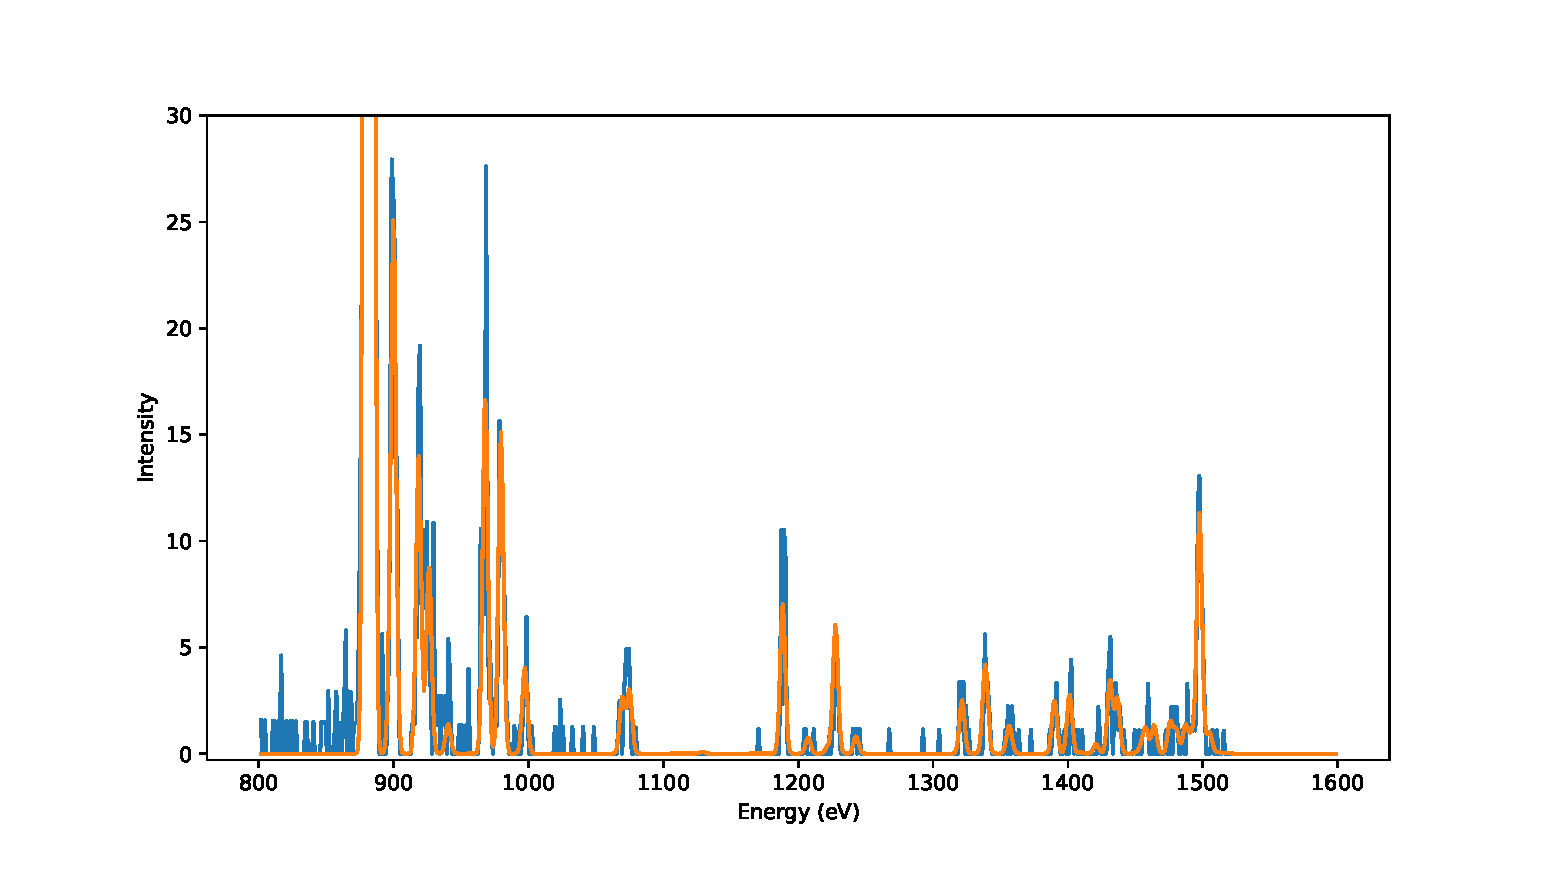
\includegraphics[width=5in]{spec_ni_h2_zoom.eps}
  \caption{\label{fig:ni+h2.zoom}Model fit to the Ni+H2 charge exchange
    spectrum showing weaker lines in more detail.}
\end{figure}
\begin{figure}
  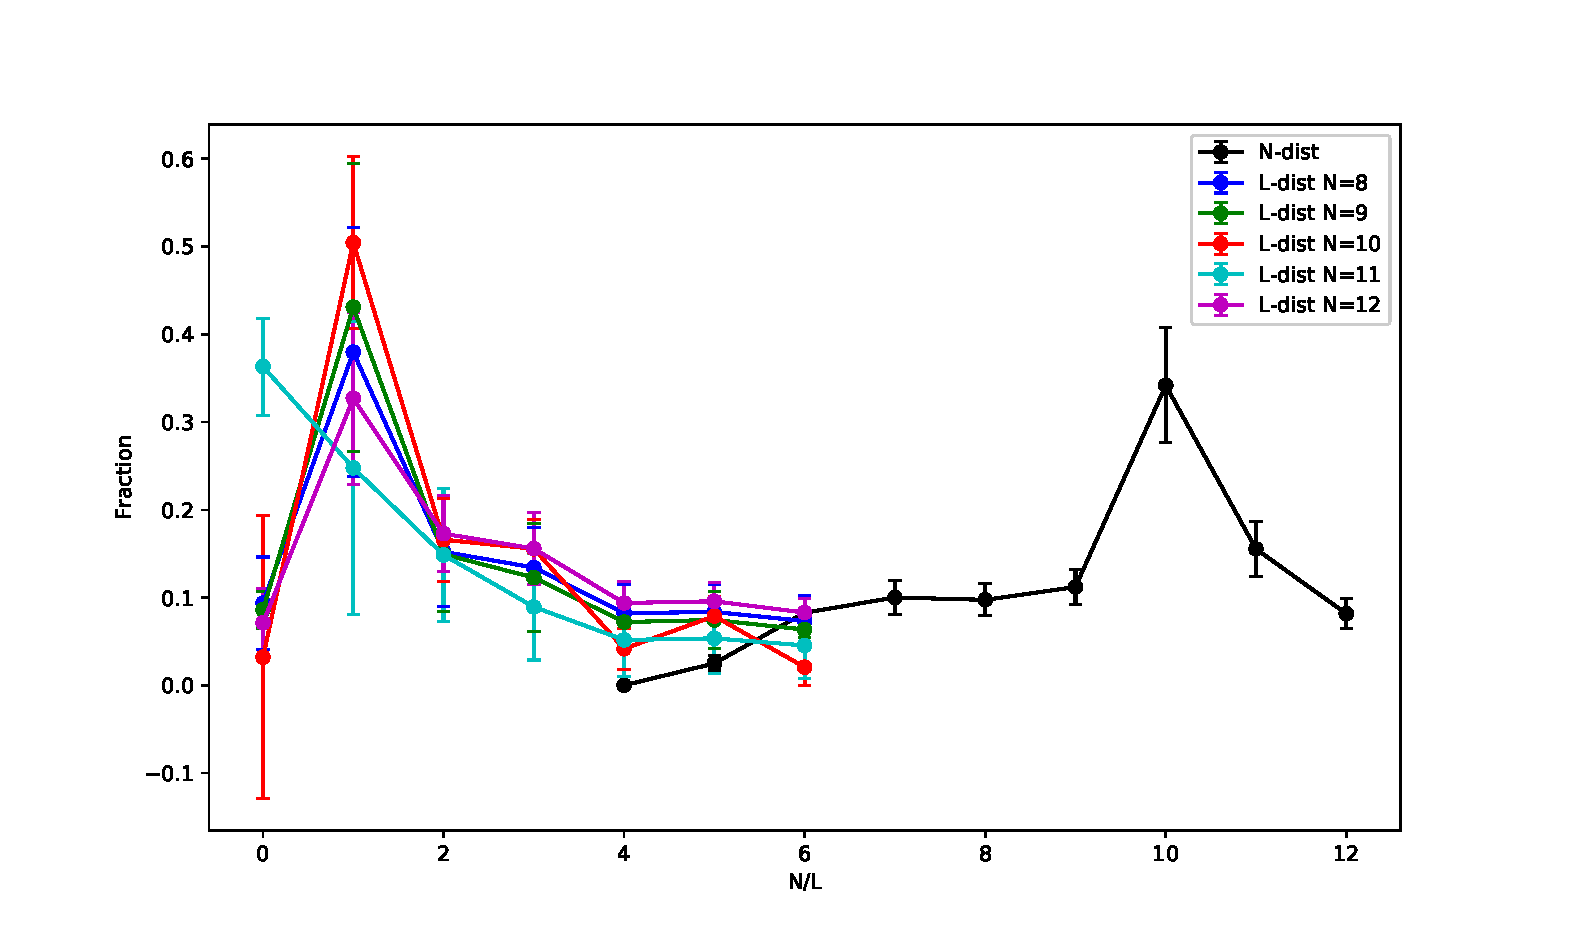
\includegraphics[width=5in]{nk_ni_h2.eps}
  \caption{\label{fig:ni+h2.nldist}Reconstructed $n$ and $l$ distributions of
    Ne-like Ni charge exchange.}
\end{figure}

\begin{figure}
  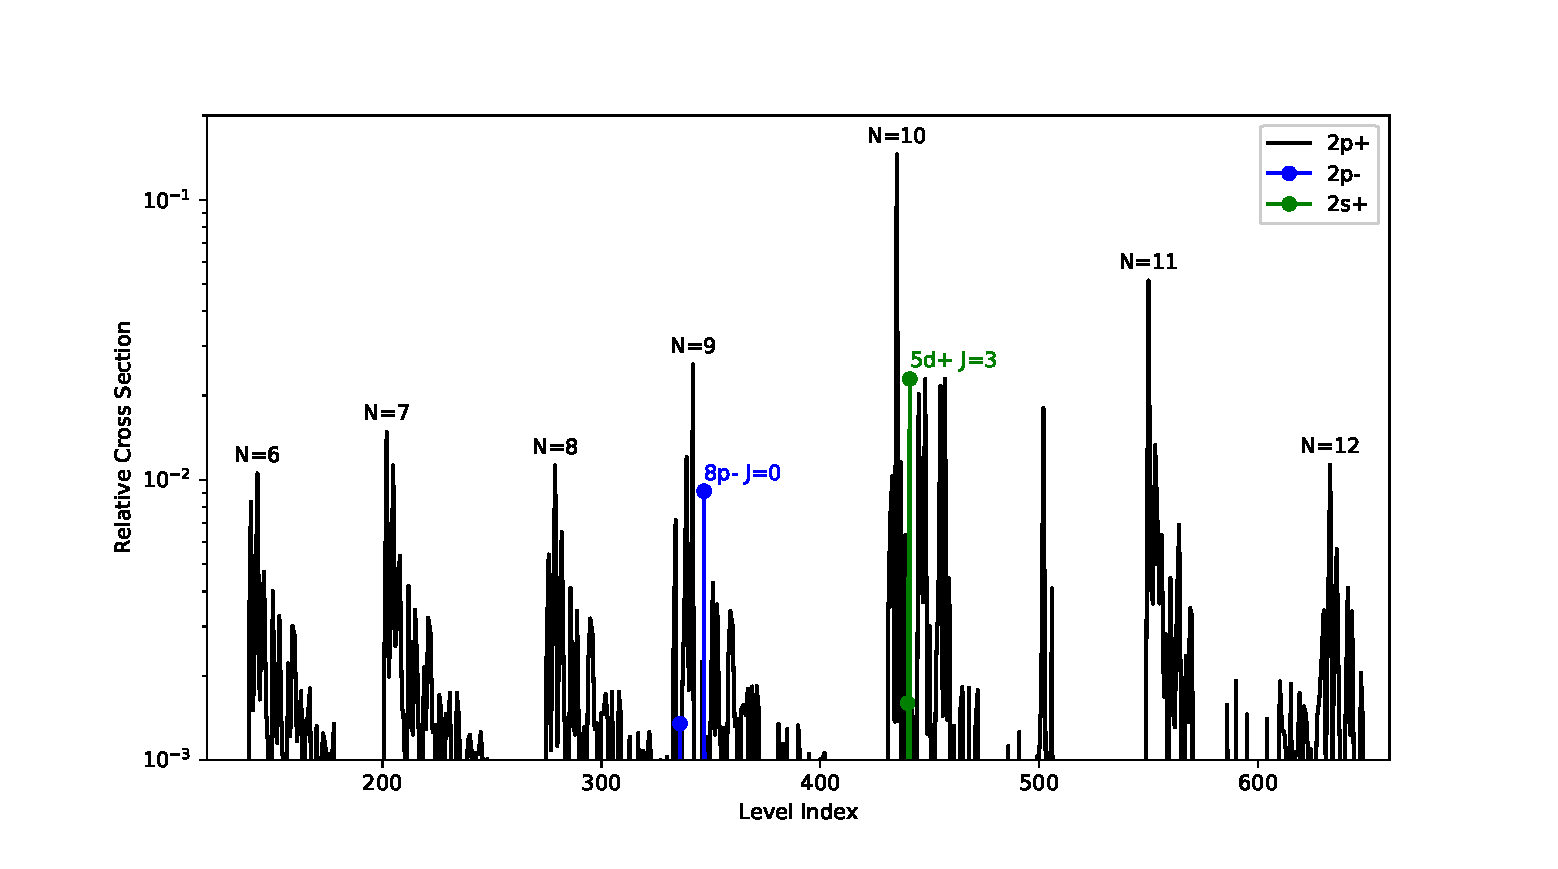
\includegraphics[width=5in]{icx_ni_h2.eps}
  \caption{\label{fig:ni+h2.icx}Relative capture cross sections of individual
    states with three core excitations of the F-like Ni.}
\end{figure}
\end{document}

